\chapter{Case study of influenza A}
\label{influenza}

\section{Abstract}

Influenza is a serious respiratory disease that causes severe illness and death in high risk populations. The rapid emergence of drug-resistant viral mutations render existing drugs void. It is thus in urgent need of new anti-influenza drugs that inhibit novel viral proteins such as nucleoprotein (NP) and the RNA-dependent RNA polymerase (RdRP) subunits PA, PB1 and PB2.

In this study, we targeted at three novel targets: the tail-loop binding domain of NP, the PB1-binding domain of PA, and the cap-binding domain of PB2. We utilized idock to perform structure-based virtual screening of 273,880 compounds, and identified several compounds that were predicted to form strong interactions with their respective protein target and believed to exhibit strong inhibitory effects. These identified compounds may serve as promising candidates for subsequent investigations \textit{in vitro} and \textit{in vivo}.

This is an ongoing collaborative project with Prof. Pang-Chui Shaw and Edwin Lo from School of Biomedical Sciences, Chinese University of Hong Kong, Hong Kong.

\section{Background}

According to the fact sheets of World Health Organization, available at http://www.who.int/mediacentre/factsheets/fs211/en/, influenza viruses have been causing sporadic pandemics and annual epidemics worldwide, every year claiming 250,000 to 500,000 lives and resulting in about 3 to 5 million cases of severe illness. The H5N1 bird flu outbreak in Hong Kong in 1997, the H1N1 swine flu outbreak in Mexico in 2009, and the ever-present threat of H5N1 acquiring human-to-human transmission capability remind us of the imminent danger posed by the influenza viruses.

Influenza viruses are negative-sense single-stranded RNA viruses. They are classified into types A, B and C based on the antigenic difference in their nucleoproteins and matrix proteins. Influenza A is the major pathogen for most cases of epidemic influenza. The influenza A genome comprises 8 segments of RNA coding for 11 proteins, which are hemagglutinin (HA), neuraminidase (NA), matrix protein 1 (M1), M2 proton channel, nucleoprotein (NP), non-structural protein 1 (NS1), nuclear export protein (NEP), polymerase acid protein (PA), polymerase basic proteins (PB1 and PB2) and PB1-F2. Influenza A viruses are further organized into 16 hemagglutinin subtypes (H1-H16) and 9 neuraminidase subtypes (N1-N9) according to their distinct antigenic properties.

The life cycle of influenza viruses has been well studied \citep{1539,1522,1525} and nearly all the viral proteins have become potential therapeutic targets \citep{1539,1519,1229,1523,1525}. To date, four anti-influenza drugs have been approved by the US FDA (Food and Drug Administration). In order of their release, they are two M2 channel blockers, amantadine (Symmetrel\textsuperscript{\textregistered}) and rimantadine (Flumadine\textsuperscript{\textregistered}), and two NA inhibitors, zanamivir (Relenza\textsuperscript{\textregistered}) and oseltamivir (Tamiflu\textsuperscript{\textregistered}). Unfortunately, oseltamivir, amantadine and rimantadine are now found to be ineffective against circulating strains due to the rapid emergence of drug-resistant viral mutations in pandemic and seasonal influenza viruses. Even worse, amantadine and rimantadine exhibit side effects on the central nervous system. No drugs have been firmly established for the other viral proteins, although leads have been proposed in some cases \citep{1229,1522,1523,1525}. These alarming facts highlight the urgent need for designing new anti-influenza drugs.
%\citep{1524} targeted host factors required for viral growth instead of viral proteins in order to circumvent drug resistance. Since the majority of the 295 host factors required for the replication of influenza virus are kinases \citep{1571}, a panel of kinase inhibitors for inhibition of influenza viral growth was screened, and the multi-kinase inhibitor ON108110 was identified to inhibit the replication of influenza A virus and other viruses including vesicular stomatitis virus (VSV) and Newcastle disease virus (NDV).%2013
%\citep{1526} screened a US drug collection of 1280 drugs, most of which have been clinically used in human or animal, for anti-influenza activity, and revealed 9 novel drug candidates for the treatment of influenza virus infection. The 9 candidates impaired different stages of influenza virus life cycle, indicating they are novel inhibitors with different mechanisms.%24 Jun 2014

%\citep{1570} The Influenza Virus Resource at the National Center for Biotechnology Information.http://www.ncbi.nlm.nih.gov/genomes/FLU/.%2008
%\citep{1569} Influenza Research Database: an integrated bioinformatics resource for influenza research and surveillance.http://www.fludb.org/.%Jan 2012
%\citep{1522} A comprehensive map of the influenza A virus replication cycle.http://www.influenza-x.org/flumap/.%2 Oct 2013

In this study we concentrate on discovering inhibitors of three influenza A proteins: NP, PA and PB2. These viral proteins are structurally related in that NP forms homo-oligomers and multiple copies of NP wrap around genomic RNA, along with a trimeric RNA-dependent RNA polymerase (RdRP) of subunits PA, PB1 and PB2 making up a ribonucleoprotein (RNP) complex.
%\citep{1568} The influenza virus RNA synthesis machine: Advances in its structure and function.%Mar 2011 review
%\citep{1579} Organization of the Influenza Virus Replication Machinery.%Dec 2012

\subsection{Nucleoprotein (NP)}

NP is the most abundantly expressed viral protein during the course of infection. NP is a polypeptide of 498 amino acids, which fold into a crescent shape with a head and a body domain. Functionally speaking, NP not only encapsidates the viral RNA, but also forms homo-oligomers. NP homo-oligomerizes by inserting the flexible tail loop (amino acids 402 to 428) into the groove of the body domain of its neighboring NP molecule.

Several crystal structures of NP have been solved. The first is a 3.2\AA\ resolution structure from human origin H1N1 (PDB ID: 2IQH) \citep{1140}. The second is a 3.3\AA\ resolution structure from avian origin H5N1 (PDB ID: 2Q06) \citep{1231}. Figure \ref{influenza:2IQH} shows the H1N1 NP crystal structure \citep{1140}, rendered by iview \citep{1366}. H5N1 NP and H1N1 NP share 94\% sequence identity \citep{1231}. Their root mean square deviation (RMSD) is 1.0\AA\ after aligning 398 residues \citep{1231}. The interaction of the tail loop of one NP molecule with the neighboring protomer in H5N1 and H1N1 is virtually identical \citep{1231}. Other more recently solved structures of H1N1 NP include 3RO5 \citep{1583}, 3TG6, 4IRY \citep{1584}, 3ZDP \citep{1573}, 4DYA, 4DYB, 4DYN, 4DYP, 4DYT and 4DYS.
%UniProt ID: Q1I2B5. A/WSN/1933 TS61 H1N1. PDB ID: 2IQH \citep{1140}.
%UniProt ID: Q9PX50. A/Chicken/Hong Kong/786/97 H5N1. PDB ID: 2Q06 \citep{1231}.
%UniProt ID: Q1K9H2. A/Wilson-Smith/1933 H1N1. PDB ID: 3RO5 \citep{1583}, 3TG6.
%UniProt ID: P15682. A/Wilson-Smith/1933 H1N1. PDB ID: 4IRY \citep{1584}, 3ZDP \citep{1573}.
%UniProt ID: B4URF1. A/WSN/1933 H1N1. PDB ID: 4DYA, 4DYB, 4DYN, 4DYP, 4DYT.
%UniProt ID: G8XKZ6. A/England/256/2009 H1N1. PDB ID: 4DYS.

\begin{figure}
\centering
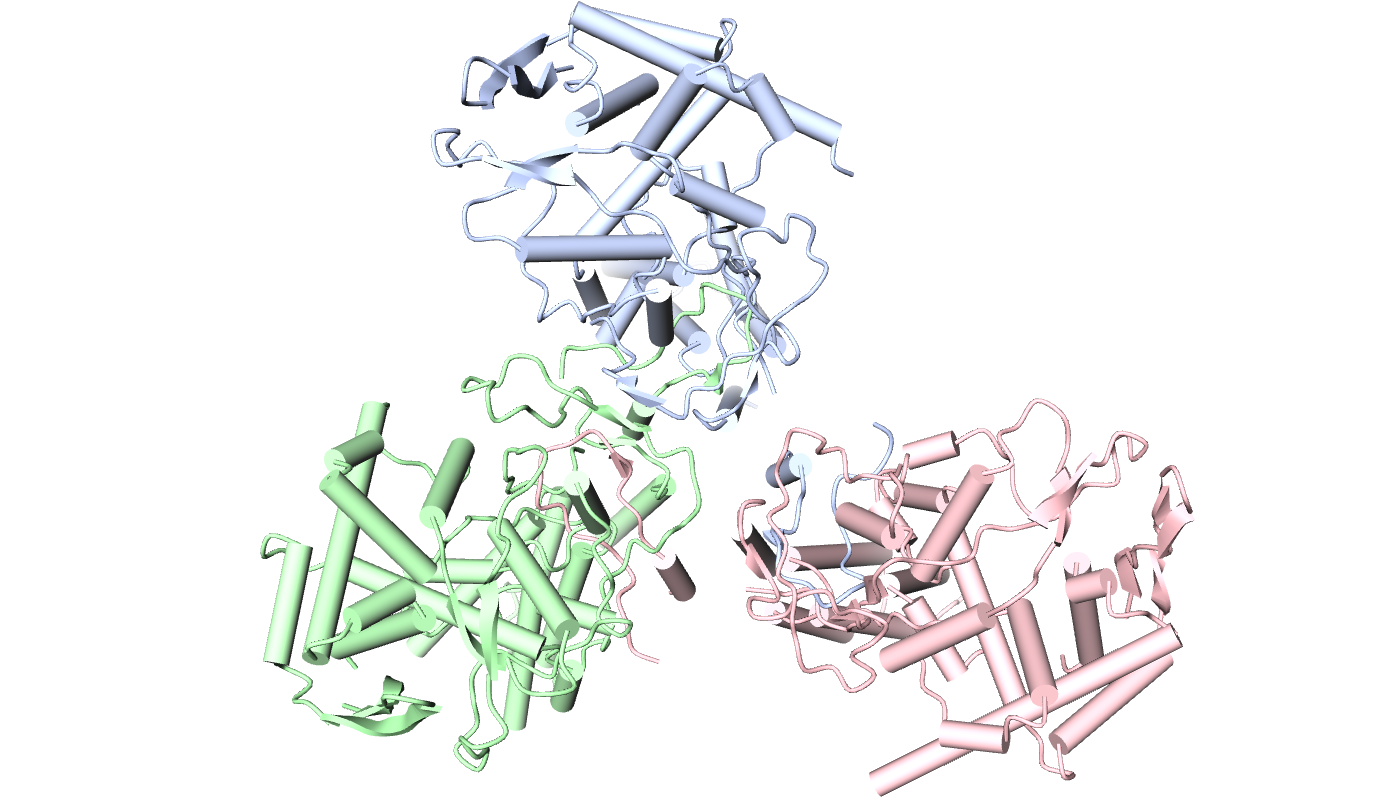
\includegraphics[width=\linewidth]{../influenza/2IQH.png}
\caption{Crystal structure of H1N1 nucleoprotein trimer with three subunits shown in different colors.}
\label{influenza:2IQH}
\end{figure}

The tail loop makes extensive interactions with the binding groove through intermolecular $\beta$-sheets, hydrophobic interactions and salt bridges \citep{1140}. Specifically at the residual level, the salt bridge between E339 lining the binding pocket and R416 on the tail loop is essential. The E339A mutant totally abolishes the RNP activities \citep{1232}. E339A and R416A are unable to support viral replication in the absence of wild type NP \citep{1233}. The R267A and E449A mutants decrease the RNP activities by more than 50\% \citep{1232}. These results indicate that within the tail-loop binding groove E339 is critical while R267 and E449 are important for NP homo-oligomerization.
%\citep{1140} Hydrophobic: A:Pro453-B:Phe420, Salt bridges: A:Glu339-B:Arg416, A:Glu449-B:Arg422.
%\citep{1231} Salt bridge: A:E449-A':R422, hydrogen bonds: B:E434-B':E434-B'':E434, salt bridge: B:K430-B:E449.
%\citep{1232} used an RNP reconstitution assay and identified eight NP single- or double-point mutants that had different degrees of defects in forming functional RNPs. These mutants were I406S, V408S P410S, R416A, L418S P419S and R422A at the tail loop, and R267A, E339A and E449A at the insertion groove. Charged residues were mutated to alanine to remove the hydrogen bond interaction, while other residues were mutated to serine to remove the hydrophobic interaction. In contrast, the T390S mutant did not show a significant change in the RNP activities. Further characterization showed that the E339A mutant existed as monomers \textit{in vitro}, and also \textit{in vivo} in the absence of RNA, deviating from the trimeric or oligomeric form of wild-type NP. Although the R267A mutant retained 45\% of the RNP activity, surprisingly it appeared as a monomer \textit{in vitro}. It resumed an oligomeric form upon the addition of RNA and retained a certain degree of RNP activity \textit{in vivo}. The E449A mutant existed as a mixture of unstable oligomers, and the R422-E449 ion pair stabilized the NP homo-oligomer.
%\citep{1447} used cryo-electron microscopy and determined the 3D structure of a biologically active recombinant RNP that reveals the NP-NP interaction domain. Mutants R416A and F412A were strongly affected in replication, whereas mutants S413T, F420A, K422A and S423A behaved as wild type. The contacts of amino acid R416 and F412 are essential for replication, while amino acid K422 does not appear to be important, in spite of being conserved among type A and B viruses.
%\citep{1561} used reverse genetics and attempted to generate 74 viruses possessing mutations at conserved amino acids of NP. Of these, 26 mutants were not viable, suggesting a critical role of the respective NP amino acids in viral replication. The 26 mutants were D72A, G93A, K113A, Y148A, R150A, R152A, R156A, R174A, R195A, R199A, R208A, R213A, E254A, A260R, K273A, K325A, A337R, E339A, R355A, R361A, A387R, Q405A, F412A, R416A, F488A, F489A.
%\citep{1574} Reverse genetics assays revealed that the R416A and Y148A mutations did not allow virus rescue.%Mar 2012
%\citep{1573} It postulated that the wild-type monomer is stabilised by phosphorylation of Ser165 and showed using biophysical measurements that a phosphomimetic mutation Ser165Asp leads to a monomeric NP. We found that serine 165 was phosphorylated and conserved in all influenza A and B viruses. The S165D mutant that mimics phosphorylation is monomeric and displays a lowered affinity for RNA compared with wt monomeric NP.%Mar 2013

The displacement of the tail loop from its binding pocket causes significant structural rearrangements in NP and completely abolishes the replication and transcription functions \citep{1231}. Tail-loop peptides are shown to disrupt NP-NP interaction and inhibit viral replication \citep{1233}. The amino acids in the tail-loop binding groove for NP oligomerization are highly conserved across 4430 sequences of NP among all influenza A virus subtypes from all hosts \citep{1513}. Therefore the tail-loop binding groove is an attractive target for inhibitor design. Chemical compounds which competitively displace the tail loop from its binding pocket would interfere with viral genome replication, and thus serve as promising candidates for anti-influenza drug development \citep{1140,1231,1232,1233}. Targeting at the tail-loop binding site, a few novel inhibitors \citep{1233} have been identified to be effective against both wild-type and mutant strains using structure-based virtual screening, but none have been approved as drugs.%\citep{1233} used structure-based virtual screening on 2IQH by Accelrys Discovery Studio.

%\citep{906} used a forward chemical genetics approach and identified NP as a druggable target and found a lead compound, nucleozin, with efficacy \textit{in vitro} and in animal studies, that triggers NP aggregation and thereby inhibits its nuclear accumulation, leading to cessation of viral replication.
%\citep{1515} developed a screening procedure to search for anti-influenza inhibitors from 1.2 million compounds, and established a high throughout virus yield reduction methodology to confirm hits. It identified previously reported anti-influenza compounds as well as new ones. Several anti-influenza compounds, including nucleozin and its analogs, were inhibitory to the influenza RNA-dependent RNA polymerase (RdRP).
%\citep{1233} reported a rational approach to target influenza virus with a new mechanism of NP-NP interaction disruption. E339A and R416A were unable to support viral replication in the absence of wild type NP, demonstrating the importance of the salt bridge between E339 lining the binding pocket and R416 on the tail loop in viral survival and establishing the salt bridge as a sensitive anti-influenza target. Peptides encompassing R416 were shown to disrupt NP-NP interaction and inhibit viral replication. Virtual screening of 1,775,422 compounds was performed to target E339...R416 and some small molecules identified were shown to disrupt the formation of NP trimers and inhibit replication of wild type and nucleozin-resistant strains.
%\citep{1583} discovered a structurally similar series of influenza replication inhibitors and show that they interfere with NP-dependent processes via formation of higher-order NP oligomers. Support for this unique mechanism is provided by site-directed mutagenesis studies, biophysical characterization of the oligomeric ligand:NP complex, and an X-ray cocrystal structure of an NP dimer of trimers (or hexamer) comprising three NP_A:NP_B dimeric subunits. Each NP_A:NP_B dimeric subunit (PDB ID: 3RO5) contains two ligands that bridge two composite, protein-spanning binding sites in an antiparallel orientation to form a stable quaternary complex. Optimization of the initial screening hit produced an analog that protects mice from influenza-induced weight loss and mortality by reducing viral titers to undetectable levels throughout the course of treatment.%13 Sep 2011
%\citep{1516} utilized nucleozin as a lead molecule and designed and synthesized a series of 1\textit{H}-1,2,3-triazole-4-carboxamide derivatives as new anti-influenza A agents targeting influenza virus nucleoproteins. Further computational studies and mechanism investigation suggested that compound 3b might directly target influenza virus A nucleoprotein to inhibit its nuclear accumulation.%Feb 2012
%\citep{1521} detailed the inhibitory mechanism of nucleozin, finding that the drug has both early- and late-acting effects on the influenza A virus life cycle. This study concluded that the primary target of nucleozin is the viral RNP, not NP. It also provided proof of the principle that influenza A virus replication can be effectively inhibited by blocking cytoplasmic trafficking of the viral genome.
%\citep{1526} indicated that the binding site for nucleozin is located close to Tyr289, which is not located close to highly conserved tail-loop binding region.
%\citep{1578} reviewed the structures of Orthomyxovirus NP, as represented by those of FluA, FluB and ISAV, and explored how the biological functions are supported by the structural features. In brief, NP in Orthomyxoviridae family show structural homology in terms of domain organization and perform essentially the same functional roles in vivo.%30 Sep 2014

\subsection{Polymerase acidic protein (PA)}

The RNA-dependent RNA polymerase is a heterotrimer composed of three subunits, namely PA, PB1 and PB2. PA contains the endonuclease domain, PB1 carries the polymerase active site, and PB2 includes the capped-RNA recognition domain. All the three subunits are required for both viral transcription and replication.% The RNA polymerase binds the conserved 3' and 5' ends of each of the 8 single-stranded RNA segments in the virus genome \citep{1192}.
%\citep{1567} Influenza A Virus Polymerase: Structural Insights into Replication and Host Adaptation Mechanisms.%Sep 2010 review

The amino-terminal residues of PB1 interact with the carboxy-terminal domain of PA. Two crystal structures of PA\textsubscript{C}-PB1\textsubscript{N} complex have been solved. The first is a 2.9\AA\ resolution structure of avian H5N1 influenza A virus PA (PA\textsubscript{C}, residues 257-716) in complex with the PA-binding region of PB1 (PB1\textsubscript{N}, residues 1-25) (PDB ID: 3CM8) \citep{1540}. The second is a 2.3\AA\ resolution structure of influenza A H1N1 (PDB ID: 2ZNL) \citep{1141}. Figure \ref{influenza:2ZNL} shows the H1N1 PA\textsubscript{C}-PB1\textsubscript{N} crystal structure, rendered by iview \citep{1366}. In addition to PA\textsubscript{C}-PB1\textsubscript{N} structures, two apo crystal structures of PA\textsubscript{C} in the absence of PB1 have been reported recently \citep{1585}. The first is a 1.9\AA\ resolution structure of H1N1 PA\textsubscript{C} (PDB ID: 4IUJ). The second is a 2.2\AA\ resolution structure of H7N9 PA\textsubscript{C} (PDB ID: 4P9A).
%UniProt ID: Q9EA60. A/environment/Hong Kong/437-6/99 H5N1. PDB ID: 3CM8 \citep{1540}.
%UniProt ID: P03433. A/Puerto Rico/8/1934 H1N1. PDB ID: 2ZNL \citep{1141}.
%UniProt ID: P15659. A/Wilson-Smith/1933 H1N1. PDB ID: 4IUJ \citep{1585}.
%UniProt ID: M9V5W3. A/chicken/Zhejiang/DTID-ZJU01/2013 H7N9. PDB ID: 4P9A \citep{1585}.

\begin{figure}
\centering
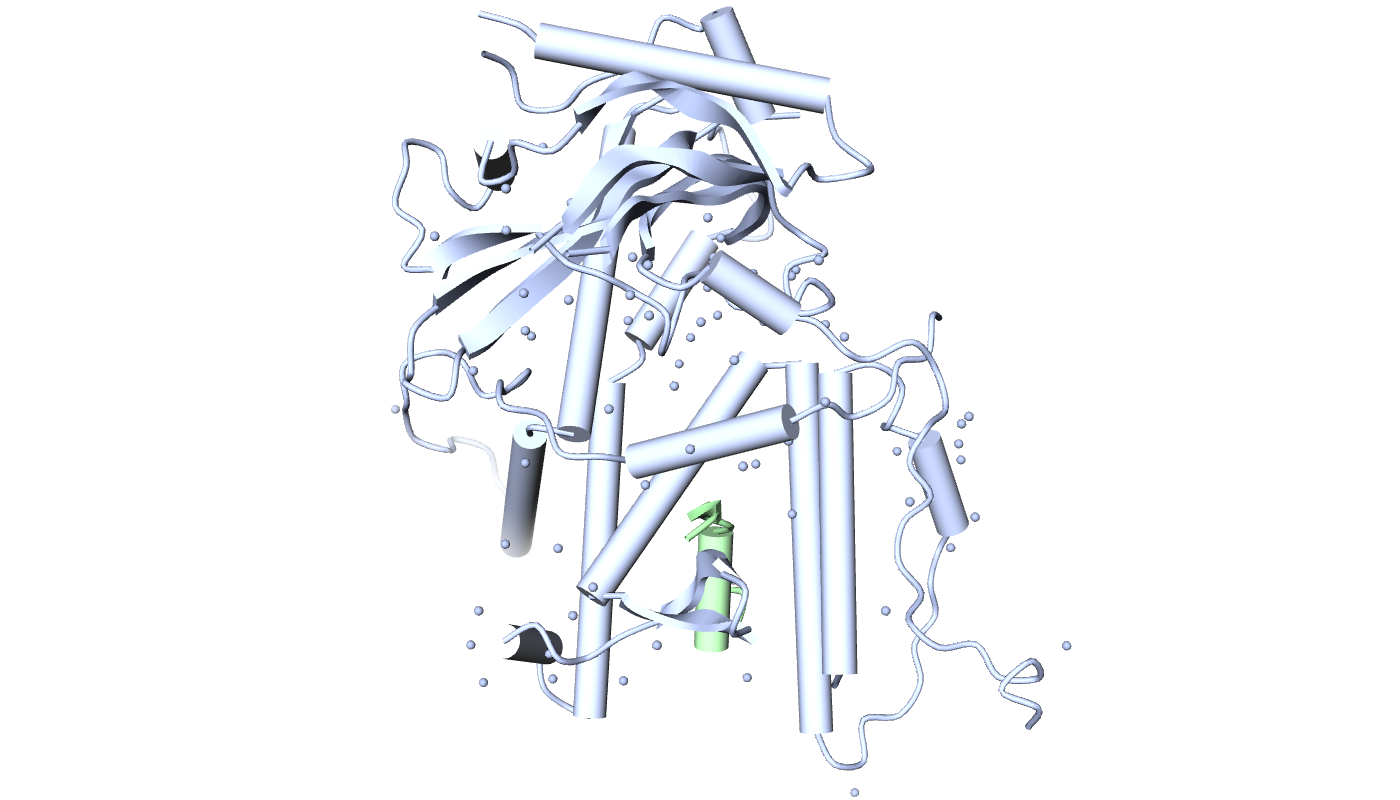
\includegraphics[width=\linewidth]{../influenza/2ZNL.png}
\caption{Crystal structure of the C-terminal domain of H1N1 PA bound to the N-terminal peptide of PB1.}
\label{influenza:2ZNL}
\end{figure}

The C-terminal domain of PA forms a deep and highly hydrophobic groove into which the N-terminal residues of PB1 can fit by forming a 3\textsubscript{10} helix P\textsubscript{5}TLLFLK\textsubscript{11} and interacting through an array of hydrogen bonds and hydrophobic contacts \citep{1141}. Four double mutations W706A/Q670A, L666G/F710E, L666G/F710G and W706A/F710Q disrupt the binding of PB1\textsubscript{N} to PA\textsubscript{C} \citep{1540}. Four point mutations V636S, L640D, L666D and W706A greatly weaken or abolish PB1 binding, and similarly reduce viral RNA synthesis in human cells \citep{1141}.
%\citep{1540} A short motif L\textsubscript{7}LFL\textsubscript{10} of PB1\textsubscript{N} interacts with the PA\textsubscript{C} hydrophobic core formed by F411, M595, L666, W706, F710, V636 and L640; PB1\textsubscript{N} residues V3 and N4 interact with PA\textsubscript{C} residue W706; V3 and D2 interact with Q408 and N412; F9, V12, P13 and A14 interact with Q670.
%\citep{1141} Most inter-subunit hydrogen bonds form through main-chain atoms of PB1. Residues Asp2 to Asn4 form anti-parallel $\beta$-sheet-like interactions with Ile621 to Glu623 of PA. The carbonyl oxygen atoms of Asp2, Val3, Phe9, Leu10 and Val12 in PB1 form hydrogen bonds to Glu623, Gln408, Trp706, Gln670 and Arg673 in PA, and the backbone nitrogen atoms of Asp2, Val3, Asn4, Leu8 and Ala14 in PB1 form hydrogen bonds with Glu 623, Asn 412, Ile 621, Pro 620 and Gln 670, respectively. Hydrophobic interactions seem to contribute substantially to the binding energy. Pro5 packs between Phe411 and Trp706, and Leu8 makes contact with the side chains of Met595, Trp619, Val636 and Leu640. To design the four point mutants, Val636 touches Leu8, Leu640 lies close to Leu8 and Pro5, Leu666 packs against the side chain of Phe9, and Trp706 interacts with Asn4, Pro5 and Thr6.

The loss of PA abolishes RNA polymerase activity and viral replication. Peptides corresponding to the PA-binding domain of PB1 block the polymerase activity and inhibits viral spread \citep{1234,1575,1541,1586}.
%\citep{1234} showed that a 25-amino-acid peptide corresponding to the PA-binding domain of PB1 inhibits the polymerase activity and viral replication, presumably by blocking the assembly of the polymerase trimer.%2007
%\citep{1575} identified an influenza A-derived peptide with a single influenza B-specific amino acid substitution which efficiently binds to PA of both virus types. This dual-binding peptide blocked the viral polymerase activity and growth of both virus types.%Oct 2009
%\citep{1541} identified high-affinity PB1-derived peptides with enhanced affinity to the PA protein of influenza A Virus polymerase.%Feb 2011
%\citep{1586} Identification of influenza virus inhibitors which disrupt of viral polymerase protein–protein interactions.%Oct 2011
The residues from PA\textsubscript{C} and PB1\textsubscript{N} at the interface are highly conserved in H1N1, H5N1 and other influenza A viruses \citep{1540,1575}.
%\citep{1540} PB1\textsubscript{N} residues interacting with PA are conserved across type A, B and C influenza viruses, and PA residues shown to interact with PB1\textsubscript{N} are similarly conserved. The high conservation of the PB1\textsubscript{N} binding site on PA suggests that anti-virals targeting this site may be less susceptible to problems of resistance.%Aug 2008
%\citep{1575} reported that the PA-binding domains of the polymerase subunits PB1 of influenza A and B viruses are highly conserved.%2009
Key interface residue mutations and PB1\textsubscript{N}-derived peptides inhibit viral replication and transcription, suggesting a crucial role of PA\textsubscript{C}-PB1\textsubscript{N} interactions in polymerase activity and heterotrimer formation. Therefore, novel chemotherapeutic agents mimicking the PB1\textsubscript{N} 3\textsubscript{10} helix are potential inhibitors of PA\textsubscript{C}-PB1\textsubscript{N} dimerization. Targeting at the PB1 binding site of PA, two FDA approved medications \citep{1576} and several novel small molecules \citep{1235,1550,1542,1587,1527} have been identified, but none have been approved as anti-influenza drugs.%\citep{1576} used structure-based virtual screening by ICM. \citep{1542} used structure-based virtual screening by Glide and Gold.  \citep{1235,1550,1527} used ligand-based virtual screening by FLAP.
%\citep{1576} There are two FDA approved medications, benzbromarone and diclazuril, that in addition to their intended use also possess anti-IAV abilities due to their structural similarity with the N terminal domain of PB1 that interacts with the C-terminus of PA.%Feb 2012
%\citep{1235} identified small molecules that disrupt the interactions between the PA and PB1 subunits of influenza virus RNA polymerase and block virus growth in cell culture. Several of these compounds showed no cytotoxicity at concentrations up to 1 mM and the most active compound blocked the formation of virus progeny with low micromolar potency. Additionally, the most active compound was effective not only against FluA but also against FluB. This compound inhibited the replication of a number of FluA virus strains, including wild type and oseltamivir-resistant strains.%Apr 2012
%\citep{1550} Structural Investigation of Cycloheptathiophene-3-carboxamide Derivatives Targeting Influenza Virus Polymerase Assembly.%Dec 2013
%\citep{1542} High-throughput docking for the identification of new influenza A virus polymerase inhibitors targeting the PA–PB1 protein–protein interaction.%Jan 2014
%\citep{1587} The Fight against the Influenza A Virus H1N1: Synthesis, Molecular Modeling, and Biological Evaluation of Benzofurazan Derivatives as Viral RNA Polymerase Inhibitors.%Jan 2014
%\citep{1527} Optimization of Small-Molecule Inhibitors of Influenza Virus Polymerase: From Thiophene-3-Carboxamide to Polyamido Scaffolds.%May 2014

\subsection{Polymerase basic protein 2 (PB2)}

Transcription of influenza virus can be divided into the following stages \citep{1236}: 1) binding of the 5' and 3' vRNA sequences to PB1, probably causing a conformational change in the polymerase complex; 2) binding of the 5' cap of a host pre-mRNA to PB2; 3) cleavage of a phosphodiester bond 10 to 13 nucleotides downstream of the cap by PA; and 4) activation of the viral mRNA transcription at the cleaved 3' end of the capped fragment.

PB2 residues 318 to 483 form the cap-binding domain, which is essential for cap-dependent transcription by viral RNPs \textit{in vitro} and \textit{in vivo}. Figure \ref{influenza:2VQZ} shows the 2.3\AA\ resolution crystal structure of the influenza A H3N2 PB2 cap-binding domain in complex with a 5'cap analog m\textsuperscript{7}GTP (PDB ID: 2VQZ) \citep{1192}, rendered by iview \citep{1366}. Other recently solved crystal structures of PB2\textsubscript{cap} include 4EQK \citep{1554}, 4NCE \citep{1558}, 4NCM \citep{1558} and 4P1U \citep{1558} for the H3N2 strain, 4ENF \citep{1554}, 3WI0 \citep{1546}, 3WI1 \citep{1546} and 4J2R \citep{1555} for the H1N1 strain, and 4ES5 \citep{1554}, 4CB4 \citep{1557}, 4CB5 \citep{1557}, 4CB6 \citep{1557} and 4CB7 \citep{1557} for the H5N1 strain.
%UniProt ID: P31345. A/Victoria/3/1975 H3N2. PDB ID: 2VQZ \citep{1192}, 4NCE \citep{1558}, 4NCM \citep{1558}, 4P1U \citep{1558}.
%UniProt ID: P03428. A/Puerto Rico/8/1934 H1N1. PDB ID: 4ENF \citep{1554}, 3WI0 \citep{1546}, 3WI1 \citep{1546}, 4J2R \citep{1555}.
%UniProt ID: Q91MB1. A/Hong Kong/1/1968 H3N2. PDB ID: 4EQK \citep{1554}.
%UniProt ID: Q4FAU9. A/Bar-headed Goose/Qinghai/12/05 H5N1. PDB ID: 4ES5 \citep{1554}.
%UniProt ID: Q2LG68. A/duck/Shantou/4610/2003 H5N1. PDB ID: 4CB4 \citep{1557}, 4CB5 \citep{1557}, 4CB6 \citep{1557}, 4CB7 \citep{1557}.
%Polymerase: 4WSB (FluA), 4WSA (FluB1), 4WRT (FluB2).

%\citep{1554} Structural and Functional Characterization of K339T Substitution Identified in the PB2 Subunit Cap-binding Pocket of Influenza A Virus. Lys339 located in the cap-binding pocket of H5N1 PB2cap was gradually replaced by Thr339 over the past decade. K339T substitution in PB2cap reduces the cap binding affinity, polymerase activity, RNA synthesis activity, and murine mortality. PDB ID: 4ENF, 4EQK, 4ES5.%Feb 2013
%\citep{1546} Conformational Polymorphism of m7GTP in Crystal Structure of the PB2 Middle Domain from Human Influenza A Virus. PDB ID: 3WI0, 3WI1.%Nov 2013
%\citep{1555} Crystallization and preliminary X-ray diffraction studies of a surface mutant of the middle domain of PB2 from human influenza A (H1N1) virus. PDB ID: 4J2R.%early 2014
%\citep{1558} Discovery of a Novel, First-in-Class, Orally Bioavailable Azaindole Inhibitor (VX-787) of Influenza PB2. PDB ID: 4NCE, 4NCM, 4P1U.%Jul 2014

\begin{figure}
\centering
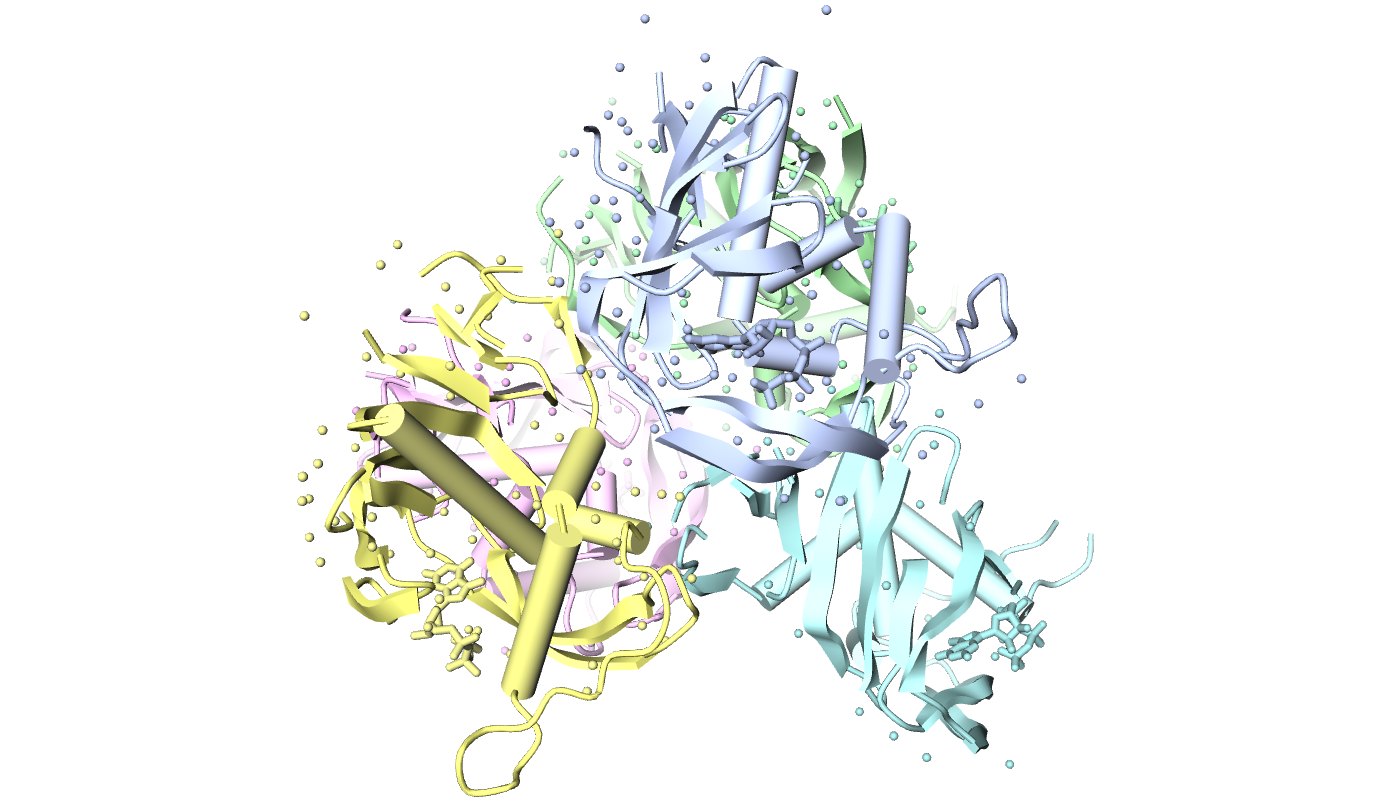
\includegraphics[width=\linewidth]{../influenza/2VQZ.png}
\caption{Crystal structure of H3N2 PB2 cap binding domain in complex with m\textsuperscript{7}GTP.}
\label{influenza:2VQZ}
\end{figure}

The binding of m\textsuperscript{7}GTP to PB2\textsubscript{cap} is assisted by a hydrophobic sandwich between the aromatic residues Phe325 and Phe404. This results in strong electrostatic interactions between the positively charged methylated base m\textsuperscript{7}G and the aromatic $\pi$-electrons, giving up to 100-fold discrimination against a nonmethylated base, i.e. m\textsuperscript{7}GTP versus GTP \citep{1192}. On the solvent side of the ligand, the sandwich is completed by His357, which stacks parallel to the base. The key acidic residue Glu361 makes hydrogen bonds with the N1 and N2 atoms of the guanine. Lys376 is involved in base recognition by interaction with O6. Phe323 stacks on the ribose. His432 and Asn429 interact with the $\alpha$-phosphate. His357, Lys339 and Arg355 interact with the $\gamma$-phosphate. Mutants E361A and K376A had no remaining affinity. Mutants F325A, H357A and F404A had greatly reduced affinity. Mutant F323A had weak binding activity \citep{1192}.
%\citep{1192} The five phenylalanines Phe404, Phe323, Phe325, Phe330 and Phe363 form a remarkable hydrophobic cluster. There are two well-ordered, buried water molecules in the ligand pocket that interact with Glu361, Lys376 and Gln406 but not directly with the ligand. Within hydrogen-bonding distance of the N2 of the base is either another water molecule or Ser320, depending on the particular molecule in the asymmetric unit. The N7 methyl group is in van der Waals contact with the side chain of Gln406 (3.4 \AA), and the carbonyl oxygen of Phe404 (3.4\AA) with the side chain of Met431, which is slightly further away. However, as previously noted, specificity for m\textsuperscript{7}G is primarily determined by the positive charge induced by methylation rather than by the additional weak interactions made by the methyl group. Unlike other cap binding proteins, PB2 has no direct interactions with either ribose hydroxyl, which are solvent exposed. The triphosphate is bent around toward the base with the $\alpha$-phosphate interacting with His432 and Asn429 and the $\gamma$-phosphate interacting with residues His357, Lys339 and Arg355.

Phe404 is conserved in B and C viruses, whereas His357, on the other side of the sandwich, is unique to influenza A and is replaced by the more conventional cap-stacking residue tryptophan in influenza B and C \citep{1192}. A statistical analysis of 13 key residues using 9246 sequences with unambiguous host annotation showed that most of the 13 residues were highly conserved, except that Lys339 and Arg355 showed polymorphisms in certain subtypes \citep{1554}.

PB2\textsubscript{cap} is structurally distinct from other cap binding proteins \citep{1192}. Hence PB2\textsubscript{cap} appears to be a favorable drug target for the development of new antiviral drugs. Targeting at the PB2\textsubscript{cap} binding site, several novel small molecules \citep{1236,1557,1558} have been identified, but none have been approved as anti-influenza drugs.
%\citep{1236} Identification of BPR3P0128 as an Inhibitor of Cap-Snatching Activities of Influenza Virus. An inhibitor of cap-snatching activities of PB2 has been identified by high-throughput screening \citep{1236}. BPR3P0128 appears to target a cellular factor associated with viral PB2 cap-snatching activity.%2012
%\citep{1557} New 7-Methylguanine Derivatives Targeting the Influenza Polymerase PB2 Cap-Binding Domain. PDB ID: 4CB4, 4CB5, 4CB6, 4CB7.%Oct 2013
%\citep{1558} Discovery of a Novel, First-in-Class, Orally Bioavailable Azaindole Inhibitor (VX-787) of Influenza PB2. PDB ID: 4NCE, 4NCM, 4P1U.%Jul 2014

%A cap mimic, if designed, would inhibit the transcription of influenza mRNAs. However, such a mimic may also be recognized by cellular cap-binding proteins and cause selectivity and cytotoxicity issues. The similar cap-binding mode of host cap-binding proteins may pose a significant challenge for overcoming cytotoxicity of such an influenza inhibitor.

%\citep{1552} showed H5N1 HK PB2 has a strong inhibitory effect on the RNP activity when introduced into the polymerase of other influenza strains of H1N1 or H3N2. HK PB1 and HK PA did not appear to have this effect.%Feb 2012
%\citep{1553} performed molecular dynamics simulations and free energy calculations on the influenza A virus PB2 subunit with a cap analog m7GTP, and showed that some key residues in the active site, such as Arg355, His357, Glu361 as well as Gln406, could offer significant hydrogen bonding and hydrophobic interactions with the guanine ring of the cap analog m7GTP to form an aromatic sandwich mechanism for the cap recognition and positioning in the active site. Subsequently, they applied this idea to a virtual screening procedure and identified 5 potential candidates that might be inhibitors against the PB2 subunit. Interestingly, 2 candidates Cpd1 and Cpd2 have been already reported to have inhibitory activities to the influenza virus cap-binding proteins. Further calculation also showed that they had comparatively higher binding affinities to the PB2 subunit than that of m7GTP.%Sep 2012
%\citep{1560} Comparative Structural and Functional Analysis of Orthomyxovirus Polymerase Cap-Snatching Domains.%Jan 2014
%\citep{1556} identified three amino acids, 147T, 339T and 588T, in PB2 that are critical for efficient replication and high virulence of an H5N1 influenza isolate, TY165, in mammalian cells.%Oct 2014

\section{Motivation}

The influenza viruses have been constantly mutating into drug-resistent strains. The four existing anti-influenza drugs gradually lose their effectiveness. New drugs targeting novel viral proteins are thus highly desired. The key residues located in the tail-loop binding groove of NP, the PB1\textsubscript{N} binding pocket of PA\textsubscript{C} and the cap-binding domain of PB2 are highly conserved, and therefore serve as attractive drug targets. Although some inhibitors have been proposed, designed, synthesized and evaluated in some cases, none have been firmly established as new anti-influenza drugs. In this study, we attempted to discover novel anti-influenza small-molecule inhibitors targeting the above three conserved sites on three viral proteins, and hopefully optimize the inhibitors into approved drugs.

\section{Objective}

We aimed at the discovery of anti-influenza small molecules. We performed structure-based virtual screening by idock \citep{1153} to select candidate molecules.

\section{Methods}

We downloaded the X-ray crystallographic structures of NP trimer (PDB ID: 2IQH) \citep{1140}, PA\textsubscript{C} in complex with PB1\textsubscript{N} (PDB ID: 2ZNL) \citep{1141}, and PB2\textsubscript{cap} in complex with m\textsuperscript{7}GTP (PDB ID: 2VQZ) \citep{1192}. For the 2IQH NP trimer structure, only chain A was retained and chains B and C were removed. For the 2ZNL PA\textsubscript{C}-PB1\textsubscript{N} structure, only PA\textsubscript{C} was retained and PB1\textsubscript{N} was removed. For the 2VQZ PB2\textsubscript{cap}-m\textsuperscript{7}GTP structure, only PB2 chain A was retained and PB2 chains B, D, E, F, and m\textsuperscript{7}GTP were removed. Table \ref{influenza:SearchSpace} lists the centers and sizes of the docking space of the three structures.

\begin{table}
\caption{Search space defined for docking the 2IQH, 2ZNL and 2VQZ structures.}
\label{influenza:SearchSpace}
\begin{tabular}{ccccccc}
\hline
PDB ID & center\_x & center\_y & center\_z & size\_x & size\_y & size\_z\\
\hline
2IQH & 82.440 & 100.261 & 26.307 & 30 & 24 & 22\\
2ZNL & -7.965 & -56.681 & 20.928 & 30 & 24 & 24\\
2VQZ & 46.857 & 24.018 & -30.614 & 16 & 14 & 18\\
\hline
\end{tabular}
\end{table}

We collected 273,880 compounds from version 2013-02-19 of the Specs catalog of the ZINC database \citep{532,1178}. The Specs compounds were chosen because they are readily available and commercially cheap.

We then executed idock v2.1.3 with a grid map granularity of 0.08\AA. Each compound was docked against the specified binding site of each of the three viral proteins, and was subsequently ranked according to the predicted idock score in kcal/mol units.

\section{Results}

\subsection{Nucleoprotein (NP)}

Table \ref{influenza:2IQH-Hits-10} lists

\begin{table}
\caption{Predicted top ten NP-tail-loop-binding-groove-targeted compounds ranked by idock score (top half) and RF-Score-v3 (bottom half).}
\label{influenza:2IQH-Hits-10}
\begin{tabular}{ccc}
\hline
ZINC ID & idock score (kcal/mol) & RF-Score-v3 (pKd)\\
\hline
08398177 & -15.78 & 8.50\\
04527915 & -14.79 & 7.54\\
08427160 & -14.51 & 8.29\\
08448951 & -14.45 & 8.62\\
08443691 & -14.40 & 8.71\\
08455791 & -14.22 & 8.49\\
08425107 & -14.16 & 8.22\\
08453194 & -14.07 & 8.10\\
08443534 & -13.99 & 8.21\\
08442491 & -13.96 & 8.37\\
\hline
08384690 &  -9.76 & 9.79\\
08384620 &  -9.25 & 9.68\\
06143179 &  -8.97 & 9.56\\
08430094 &  -9.08 & 9.35\\
08432234 &  -8.18 & 9.32\\
08384589 & -10.31 & 9.30\\
08399495 & -10.01 & 9.27\\
08399544 & -10.35 & 9.24\\
08399490 & -10.09 & 9.21\\
08384414 & -10.66 & 9.20\\
\hline
\end{tabular}
\end{table}

Figure \ref{influenza:2IQH-Hits-4} visualizes the predicted structures of NP in complex of the top four compounds ranked by idock score and RF-Score-v3.

\begin{figure}
\centering
\subfloat[ZINC08398177.]
{
  \includegraphics[width=0.48\linewidth]{../influenza/2IQH-ZINC08398177-ms.png}
}
\subfloat[ZINC04527915.]
{
  \includegraphics[width=0.48\linewidth]{../influenza/2IQH-ZINC04527915-ms.png}
}
\\
\subfloat[ZINC08427160.]
{
  \includegraphics[width=0.48\linewidth]{../influenza/2IQH-ZINC08427160-ms.png}
}
\subfloat[ZINC08448951.]
{
  \includegraphics[width=0.48\linewidth]{../influenza/2IQH-ZINC08448951-ms.png}
}
\\
\subfloat[ZINC08384690.]
{
  \includegraphics[width=0.48\linewidth]{../influenza/2IQH-ZINC08384690-ms.png}
}
\subfloat[ZINC08384620.]
{
  \includegraphics[width=0.48\linewidth]{../influenza/2IQH-ZINC08384620-ms.png}
}
\\
\subfloat[ZINC06143179.]
{
  \includegraphics[width=0.48\linewidth]{../influenza/2IQH-ZINC06143179-ms.png}
}
\subfloat[ZINC08430094.]
{
  \includegraphics[width=0.48\linewidth]{../influenza/2IQH-ZINC08430094-ms.png}
}
\caption{Predicted structures of NP in complex of the top four compounds ranked by idock score (a to d) and RF-Score-v3 (e to h).}
\label{influenza:2IQH-Hits-4}
\end{figure}

\subsection{Polymerase acidic protein (PA)}

Table \ref{influenza:2ZNL-Hits-10} lists

\begin{table}
\caption{Predicted top ten PA\textsubscript{C}-targeted compounds ranked by idock score (top half) and RF-Score-v3 (bottom half).}
\label{influenza:2ZNL-Hits-10}
\begin{tabular}{ccc}
\hline
ZINC ID & idock score (kcal/mol) & RF-Score-v3 (pKd)\\
\hline
08383903 & -15.45 & 8.24\\
08398361 & -14.53 & 8.01\\
08417364 & -14.09 & 8.53\\
04176726 & -13.85 & 7.96\\
16526187 & -13.84 & 7.57\\
00652029 & -13.79 & 7.84\\
08453194 & -13.76 & 8.01\\
08427363 & -13.67 & 7.16\\
08444058 & -13.61 & 8.24\\
04527916 & -13.49 & 8.05\\
\hline
08439610 & -11.20 & 8.90\\
08396899 & -10.81 & 8.88\\
08384461 &  -9.75 & 8.84\\
08443595 & -11.59 & 8.83\\
08399680 &  -9.78 & 8.77\\
08454594 & -11.78 & 8.74\\
08399439 & -10.26 & 8.72\\
08442229 & -10.21 & 8.71\\
08398784 & -10.88 & 8.70\\
08397557 & -11.66 & 8.69\\
\hline
\end{tabular}
\end{table}

Figure \ref{influenza:2ZNL-Hits-4} visualizes the predicted structures of PA\textsubscript{C} in complex of the top four compounds ranked by idock score and RF-Score-v3.

\begin{figure}
\centering
\subfloat[ZINC08383903.]
{
  \includegraphics[width=0.48\linewidth]{../influenza/2ZNL-ZINC08383903-ms.png}
}
\subfloat[ZINC08398361.]
{
  \includegraphics[width=0.48\linewidth]{../influenza/2ZNL-ZINC08398361-ms.png}
}
\\
\subfloat[ZINC08417364.]
{
  \includegraphics[width=0.48\linewidth]{../influenza/2ZNL-ZINC08417364-ms.png}
}
\subfloat[ZINC04176726.]
{
  \includegraphics[width=0.48\linewidth]{../influenza/2ZNL-ZINC04176726-ms.png}
}
\\
\subfloat[ZINC08439610.]
{
  \includegraphics[width=0.48\linewidth]{../influenza/2ZNL-ZINC08439610-ms.png}
}
\subfloat[ZINC08396899.]
{
  \includegraphics[width=0.48\linewidth]{../influenza/2ZNL-ZINC08396899-ms.png}
}
\\
\subfloat[ZINC08384461.]
{
  \includegraphics[width=0.48\linewidth]{../influenza/2ZNL-ZINC08384461-ms.png}
}
\subfloat[ZINC08443595.]
{
  \includegraphics[width=0.48\linewidth]{../influenza/2ZNL-ZINC08443595-ms.png}
}
\caption{Predicted structures of PA\textsubscript{C} in complex of the top four compounds ranked by idock score (a to d) and RF-Score-v3 (e to h).}
\label{influenza:2ZNL-Hits-4}
\end{figure}

\subsection{Polymerase basic protein 2 (PB2)}

Table \ref{influenza:2VQZ-Hits-10} lists

\begin{table}
\caption{Predicted top ten PB2\textsubscript{cap}-targeted compounds ranked by idock score (top half) and RF-Score-v3 (bottom half).}
\label{influenza:2VQZ-Hits-10}
\begin{tabular}{ccc}
\hline
ZINC ID & idock score (kcal/mol) & RF-Score-v3 (pKd)\\
\hline
08383936 & -12.52 & 7.67\\
08386295 & -12.15 & 7.41\\
03015113 & -11.85 & 7.67\\
15188425 & -11.74 & 7.53\\
02125231 & -11.69 & 7.09\\
02154274 & -11.56 & 7.31\\
08453194 & -11.56 & 7.40\\
02077599 & -11.46 & 7.21\\
02077477 & -11.45 & 7.36\\
00657519 & -11.45 & 7.65\\
\hline
08439610 &  -8.77 & 8.47\\
08439605 &  -8.59 & 8.38\\
08399683 &  -7.38 & 8.37\\
08437929 &  -9.27 & 8.33\\
08455074 &  -9.81 & 8.25\\
08444191 &  -9.56 & 8.23\\
08446351 &  -9.96 & 8.20\\
08452812 &  -9.49 & 8.20\\
02752464 & -10.58 & 8.19\\
08446353 &  -8.82 & 8.19\\
\hline
\end{tabular}
\end{table}

Figure \ref{influenza:2VQZ-Hits-4} visualizes the predicted structures of PB2\textsubscript{cap} in complex of the top four compounds ranked by idock score and RF-Score-v3.

\begin{figure}
\centering
\subfloat[ZINC08383936.]
{
  \includegraphics[width=0.48\linewidth]{../influenza/2VQZ-ZINC08383936-ms.png}
}
\subfloat[ZINC08386295.]
{
  \includegraphics[width=0.48\linewidth]{../influenza/2VQZ-ZINC08386295-ms.png}
}
\\
\subfloat[ZINC03015113.]
{
  \includegraphics[width=0.48\linewidth]{../influenza/2VQZ-ZINC03015113-ms.png}
}
\subfloat[ZINC15188425.]
{
  \includegraphics[width=0.48\linewidth]{../influenza/2VQZ-ZINC15188425-ms.png}
}
\\
\subfloat[ZINC08439610.]
{
  \includegraphics[width=0.48\linewidth]{../influenza/2VQZ-ZINC08439610-ms.png}
}
\subfloat[ZINC08439605.]
{
  \includegraphics[width=0.48\linewidth]{../influenza/2VQZ-ZINC08439605-ms.png}
}
\\
\subfloat[ZINC08399683.]
{
  \includegraphics[width=0.48\linewidth]{../influenza/2VQZ-ZINC08399683-ms.png}
}
\subfloat[ZINC08437929.]
{
  \includegraphics[width=0.48\linewidth]{../influenza/2VQZ-ZINC08437929-ms.png}
}
\caption{Predicted structures of PB2\textsubscript{cap} in complex of the top four compounds ranked by idock score (a to d) and RF-Score-v3 (e to h).}
\label{influenza:2VQZ-Hits-4}
\end{figure}

\section{Discussion}

Duplicate top compound
Discuss Nrot

\section{Conclusions}

Treatment of seasonal and pandemic influenza is currently limited by the availability of only few drugs that are challenged by emergence of drug-resistant mutants.

\section{Future works}

The top scoring compounds will be subjected to post-screening evaluations, including Lipinski's rule filter, visual inspection and consensus docking \citep{1590} using DOCK \citep{1222}, AutoDock Vina \citep{595}, or PLANTS \citep{610,607,779}. The commercially available compounds will be purchased for subsequent biological evaluations.

The cytotoxicity of the compounds will first be tested by MTT assay. Influenza RNP (ribonucleoprotein) reconstitution assay will then be performed to investigate their ability to inhibit RNP transcriptional activity. Hit compounds causing significant reduction of RNP activity will be subjected to whole virus assay including plaque reduction assay and yield reduction assay using seasonal flu viruses. Surface plasmon resonance will also be performed to test the \textit{in vitro} binding affinity of the compounds to the target protein. 

For compounds that exhibit substantial anti-influenza properties, chemical analogues will be purchased for further evaluation. Structure activity relationship study will be performed to further characterize the interaction between the compound and the target protein.

Pure computational studies of prospective virtual screening for a target protein of interest, such as the methyltransferase of the dengue virus \citep{1435}, can be accepted for publication in some journals.

Recently, two apo crystal structures of H1N1 and H7N9 PA\textsubscript{C} (PDB ID: 4IUJ, 4P9A) in the absence of PB1 have been reported to exhibit the same global topology as other strains, but differ extensively in the PB1 binding pocket \citep{1585}. These structural changes demonstrate plasticity in the PA\textsubscript{C}-PB1\textsubscript{N} binding interface, which can be exploited in the development of novel therapeutic drugs.

\chapterend
